\documentclass[10pt,conference]{IEEEtran}
% Do not modify IEEEtran.cls (NCC rule). Adding packages here is fine.

\usepackage{cite}
\usepackage{amsmath,amssymb}
\usepackage{graphicx}
\usepackage{algorithm}
\usepackage{algpseudocode}
\usepackage{xcolor}
\usepackage{array}
\usepackage{placeins}
\usepackage{capt-of}
\usepackage{float}
\usepackage{balance}

\setlength{\textfloatsep}{7pt plus 2pt minus 2pt}
\setlength{\floatsep}{5pt plus 1pt minus 1pt}
\setlength{\intextsep}{6pt plus 1pt minus 1pt}
\setlength{\dbltextfloatsep}{7pt plus 2pt minus 2pt}
\setlength{\dblfloatsep}{5pt plus 1pt minus 1pt}
\setlength{\abovedisplayskip}{5pt plus 2pt minus 2pt}
\setlength{\belowdisplayskip}{5pt plus 2pt minus 2pt}
\setlength{\abovedisplayshortskip}{3pt plus 1pt}
\setlength{\belowdisplayshortskip}{3pt plus 1pt}

% Keep two-column float pages top-aligned instead of stretching gaps.
\makeatletter
\setlength{\@dblfptop}{0pt}
\setlength{\@dblfpsep}{8pt plus 2pt minus 2pt}
\setlength{\@dblfpbot}{0pt plus 1fil}
\setlength{\@fptop}{0pt}
\setlength{\@fpsep}{8pt plus 2pt minus 2pt}
\setlength{\@fpbot}{0pt plus 1fil}
\makeatother

%%%%%%%%%%%%%%%%%%%%%%%%%%%%%%%%%%%%%%%%%%%%%%%%%%%%%%%%%%%%%%%%%%%%%%%%%%%%%%
% DRAFTING HELPERS: delete these (and every \todo / \XX / \figbox) before submission
\newcommand{\todo}[1]{\textcolor{red}{[TODO: #1]}}
\newcommand{\XX}{\textcolor{red}{XX}}
\newcommand{\figbox}[2]{% placeholder figure: #1 = what goes here, #2 = height
	\fbox{\parbox[c][#2][c]{0.95\linewidth}{\centering\footnotesize\textcolor{red}{#1}}}}
%%%%%%%%%%%%%%%%%%%%%%%%%%%%%%%%%%%%%%%%%%%%%%%%%%%%%%%%%%%%%%%%%%%%%%%%%%%%%%

% Notation
\newcommand{\vect}[1]{\mathbf{#1}}
\newcommand{\Gt}{\tilde{\mathbf{G}}}
\DeclareMathOperator{\sinc}{sinc}

\begin{document}
	
	\title{Development of a GPU-Accelerated Method of Moments Solver for EM Analysis of Metasurfaces}
	
	% DOUBLE-BLIND: keep this anonymous for the review version.
	% Real names/affiliations go in only for the camera-ready version.
	% Uses the current IEEEtran author macros; the fallback below covers older
	% IEEEtran versions that only have \authorblockN / \authorblockA.
	\providecommand{\IEEEauthorblockN}[1]{\authorblockN{#1}}
	\providecommand{\IEEEauthorblockA}[1]{\authorblockA{#1}}
	\author{\IEEEauthorblockN{.}
		\IEEEauthorblockA{.}}
	
	\maketitle
	
	%==============================================================================
	\begin{abstract}
		Periodic metasurfaces printed on grounded dielectric substrates are
		commonly used as radar-absorbing surfaces and are typically designed using
		repeated evaluations of the reflection coefficient $S_{11}$ as a function
		of frequency. Although full-wave finite-element method (FEM) simulations
		with periodic boundary conditions are accurate, they are too slow for the
		extensive parameter sweeps required to build datasets for data-driven
		design. This paper presents a spectral-domain method of moments (MoM)
		solver in which the substrate and ground plane are incorporated into
		closed-form TE/TM Floquet Green's functions. The MoM operator is applied
		with fast Fourier transforms, so the dense impedance matrix is never
		explicitly formed, and the resulting system is solved with a restarted
		GMRES iteration that runs entirely on the GPU. Independent frequency
		points are distributed across multiple GPUs. For four representative
		absorber geometries, principal resonant notches agree with a
		commercial FEM solver to within $4.8\%$ in frequency. A full
		frequency sweep on the HPC A100 GPU is up to $50\times$ faster than the
		same matrix-free FFT-MoM implemented in NumPy/SciPy (complex128) on the
		CPU.
	\end{abstract}
	
	%==============================================================================
	\section{Introduction}
	
	Frequency selective surfaces (FSSs) and metasurfaces are periodic arrays of
	patterned conductors whose reflection and transmission change with
	frequency \cite{munk2000}. When the pattern is printed on a dielectric slab
	with a ground plane underneath, no power is transmitted, so whatever is not
	reflected is absorbed. Near resonance this absorption becomes strong and
	appears as a notch in the reflection coefficient $S_{11}$. Radar-absorbing
	surfaces of this kind are used to reduce radar cross-section and to control
	electromagnetic interference \cite{joy2021}. The frequency, depth and width of
	each notch are all set by the geometry of the unit cell.
	
	Designing an absorber therefore comes down to predicting $S_{11}(f)$ for many
	candidate geometries. In practice this is done with a commercial full-wave
	solver, for example the frequency-domain finite-element method (FEM) solver in
	CST Studio Suite \cite{cst}, on a single unit cell with periodic boundaries
	and Floquet ports. Each of the four cells below takes 29--199~s in CST
	(Table~\ref{tab:perf}), which is acceptable for a few hand-tuned designs but
	not for the thousands of evaluations needed to train a surrogate or
	inverse-design model \cite{liu2018,ma2018}.
	
	For planar periodic structures, the method of moments (MoM) \cite{harrington}
	avoids much of this cost. Only the metal pattern has to be discretized, since
	the substrate and ground plane can be included analytically through a
	spectral-domain Green's function \cite{itoh1980,mittra1988}. If the pattern is
	meshed on a uniform grid, the MoM operator can be applied with fast Fourier
	transforms (FFTs) instead of being stored as a dense impedance matrix
	\cite{cwik1987}. Conventional (RWG) MoM matrix assembly and factorization
	have also been accelerated on GPUs \cite{lezar2010}. These techniques have
	mostly been studied separately, and relatively little work has combined
	them in a GPU solver set up for sweeping many absorber geometries and
	frequencies.
	
	In this paper we combine them in a single solver designed for throughput,
	that is, for evaluating many geometries and frequency points quickly rather
	than for solving one very large problem. Our main contributions are:
	\begin{itemize}
		\item A spectral-domain MoM formulation for impedance-sheet patterns on a
		grounded substrate. The slab and ground plane enter through closed-form
		TE/TM Floquet Green's functions, and the operator is evaluated with FFTs,
		so memory grows linearly with the number of grid cells instead of with the
		square of the number of unknowns.
		\item A GPU implementation in which the restarted GMRES solve runs entirely
		on the device, with frequency points distributed across multiple GPUs in
		contiguous blocks and no communication between them.
		\item Validation against CST for four absorber geometries, GMRES
		iteration counts across the sweep, and runtime measurements on the HPC
		A100 GPU, showing a speedup of up to $50\times$ over the same FFT-MoM on
		the CPU (NumPy/SciPy, complex128).
	\end{itemize}
	
	%==============================================================================
	\section{Formulation}
	\label{sec:form}
	% Budget: ~1.2 pages.
	
	\subsection{Structure and Boundary Condition}
	
	Consider a doubly periodic array with periods $a=b=10$~mm in the plane
	$z=0$, printed on a substrate of thickness $h$, relative permittivity
	$\epsilon_r$ and loss tangent $\tan\delta$, and backed by a PEC ground plane
	at $z=-h$ (Fig.~\ref{fig:geometry}). We assume an $e^{j\omega t}$ time
	convention and write $\epsilon_c=\epsilon_r(1-j\tan\delta)$; $k_0$ and
	$\eta_0$ are the free-space wavenumber and impedance. The metal
	pattern $S$ is a zero-thickness sheet with surface impedance $Z_s$, which is
	zero for PEC, $(1+j)\sqrt{\omega\mu_0/2\sigma}$ for copper, and a real sheet
	resistance $R_s$ for resistive films. A $y$-polarized plane wave of
	amplitude $E_0$ is normally incident from $z>0$.
	
	Without the pattern, the grounded slab acts as a short-circuited line and
	reflects with
	\begin{equation}
		\Gamma_{\mathrm{bare}}=\frac{Z_{\mathrm{in}}-\eta_0}{Z_{\mathrm{in}}+\eta_0},
		\qquad
		Z_{\mathrm{in}}=j\frac{\eta_0}{\sqrt{\epsilon_c}}\tan\!\big(k_0\sqrt{\epsilon_c}\,h\big),
		\label{eq:gbare}
	\end{equation}
	so the tangential field at $z=0$ is
	$\vect{E}^{\mathrm{bare}}=(1+\Gamma_{\mathrm{bare}})E_0\hat{\vect{y}}$.
	The current $\vect{J}$ on $S$ radiates a scattered field
	$\vect{E}^{s}[\vect{J}]$ in the presence of the slab, and on the pattern
	\begin{equation}
		\vect{E}^{\mathrm{bare}}_t+\vect{E}^{s}_t[\vect{J}]=Z_s\vect{J},
		\qquad \vect{r}\in S.
		\label{eq:ibc}
	\end{equation}
	
	\begin{figure}[t]
		\centering
		\figbox{Fig.~1. (a) Cross-section: patterned sheet at $z=0$, substrate
			($\epsilon_r$, $\tan\delta$, $h$), PEC ground at $z=-h$, incident and reflected
			waves. (b) The four $10\times10$~mm unit-cell masks G1--G4
			(\texttt{253\_img}, \texttt{424\_img}, \texttt{82\_img}, \texttt{100\_img}).}{2.6cm}
		\caption{(a) Layered unit-cell model. (b) Unit-cell geometries G1--G4
			(white $=$ metal).}
		\label{fig:geometry}
	\end{figure}
	
	\subsection{Floquet Expansion and Spectral Green's Function}
	
	Because the structure is periodic, the current and scattered field are
	expanded in Floquet harmonics, which at normal incidence have wavenumbers
	$k_{xm}=2\pi m/a$ and $k_{yn}=2\pi n/b$, with $k_t^2=k_{xm}^2+k_{yn}^2$.
	The tangential scattered field at
	$z=0$ is
	\begin{equation}
		\vect{E}^{s}_t(x,y)=\frac{1}{ab}\sum_{m,n}
		\Gt(k_{xm},k_{yn})\,\tilde{\vect{J}}(k_{xm},k_{yn})\,
		e^{-j(k_{xm}x+k_{yn}y)},
		\label{eq:floquet}
	\end{equation}
	where $\tilde{\vect{J}}$ is the Fourier transform of $\vect{J}$ over one unit
	cell.
	
	Each harmonic splits into a TM part (along $\hat{\vect{k}}_t$) and a TE part
	(along $\hat{\vect{z}}\times\hat{\vect{k}}_t$). Each part sees the air
	half-space in parallel with the short-circuited substrate line, so its modal
	Green's function is
	\begin{equation}
		G^{\alpha}=\frac{1}{Y^{\alpha}_0-jY^{\alpha}_1\cot(k_{z1}h)},
		\qquad \alpha\in\{\mathrm{TE},\mathrm{TM}\},
		\label{eq:gmodal}
	\end{equation}
	where $Y^{\mathrm{TE}}_i=k_{zi}/(\omega\mu_0)$ and
	$Y^{\mathrm{TM}}_i=\omega\epsilon_0\epsilon_{r,i}/k_{zi}$ are the modal
	admittances of air ($i=0$, $\epsilon_{r,0}=1$) and substrate ($i=1$,
	$\epsilon_{r,1}=\epsilon_c$). The vertical wavenumbers are
	$k_{zi}=\sqrt{\epsilon_{r,i}k_0^2-k_t^2}$ with $\Im\{k_{zi}\}\le0$
	(and $\Re\{k_{zi}\}\ge0$ when real). A superstrate (here of the same $\epsilon_c$
	and $h$) only replaces $Y^{\alpha}_0$ by the admittance looking up into it.
	In Cartesian form,
	\begin{equation}
		\Gt=\frac{1}{k_t^2}
		\begin{pmatrix}
			k_x^2G^{\mathrm{TM}}+k_y^2G^{\mathrm{TE}} & k_xk_y(G^{\mathrm{TM}}-G^{\mathrm{TE}})\\
			k_xk_y(G^{\mathrm{TM}}-G^{\mathrm{TE}}) & k_y^2G^{\mathrm{TM}}+k_x^2G^{\mathrm{TE}}
		\end{pmatrix},
		\label{eq:gdyad}
	\end{equation}
	which reduces to $G^{\mathrm{TE}}\mathbf{I}$ at $k_t=0$. Dielectric loss and
	the PEC ground are thus included in $\Gt$ rather than as extra unknowns.
	
	\subsection{Discretization}
	
	The unit cell is divided into an $N\times N$ grid of square cells of side
	$\Delta=a/N$, and the pattern is represented by its metal cells
	(Fig.~\ref{fig:geometry}b). The current is expanded in $x$- and $y$-directed
	rooftop basis functions $\vect{f}_p$ \cite{glisson1980} on the interior
	edges of the metal. An $x$-directed rooftop is triangular in $x$ over two
	adjacent cells and constant in $y$ over one cell, so its transform is
	separable,
	\begin{equation}
		\tilde{F}^x_p=\Delta^2\sinc^2\!\left(\tfrac{k_x\Delta}{2}\right)
		\sinc\!\left(\tfrac{k_y\Delta}{2}\right)e^{j(k_xx_p+k_yy_p)},
	\end{equation}
	with $\sinc(u)=\sin u/u$ (and likewise for $y$). Galerkin testing of
	\eqref{eq:ibc} gives the $N_u\times N_u$ system
	\begin{equation}
		\vect{A}\vect{I}=\vect{v},\quad \vect{A}=Z_s\vect{T}-\vect{Z},\quad
		Z_{pq}=\frac{1}{ab}\sum_{m,n}\tilde{\vect{F}}_p^{*}\cdot\Gt\,\tilde{\vect{F}}_q,
		\label{eq:system}
	\end{equation}
	where $\vect{T}$ is the Gram matrix of the basis and
	$v_p=\langle\vect{f}_p,\vect{E}^{\mathrm{bare}}\rangle$.
	
	\subsection{Reflection Coefficient}
	
	The specular reflection is carried by the $(0,0)$ harmonic. Referenced to
	the sheet plane $z=0$,
	\begin{equation}
		S_{11}=\Gamma_{\mathrm{bare}}+\frac{T_{\mathrm{scat}}}{E_0\,ab}\,
		\hat{\vect{y}}\cdot\Gt(0,0)\,\tilde{\vect{J}}(0,0),
		\label{eq:s11}
	\end{equation}
	where $T_{\mathrm{scat}}=1$ for air above the sheet and is a scalar factor
	when a superstrate is present. Only co-polarized reflection is computed. A
	constant phase offset may remain relative to a CST Floquet port whose
	reference plane is not $z=0$; it does not affect $|S_{11}|$, which is the
	quantity compared below.
	
	%==============================================================================
	\section{GPU-Accelerated Solver}
	\label{sec:gpu}
	% Budget: ~1.3 pages. This is the core contribution; give it the most care.
	
	\subsection{FFT-Based Operator Application}
	
	Because the basis functions sit on a uniform grid and the Green's function is
	periodic, $\vect{Z}$ extended to the full grid is block circulant. Its product
	with a vector is therefore a spectral-domain multiplication followed by
	restriction to the metal edges (Algorithm~\ref{alg:matvec}), as in the CG-FFT
	approach \cite{cwik1987}. The spectral kernels
	$\tilde{K}_{uv}=\frac{1}{ab}\tilde{F}^{u*}\tilde{G}_{uv}\tilde{F}^{v}$ are
	computed once per frequency on an $N\times N$ FFT grid ($M=N$). Floquet
	harmonics with $|m|$ or $|n|$ beyond $N/2$ are not stored separately; they
	are folded onto this grid by aliasing, which is the discrete Green's-function
	sum used throughout.
	
	\begin{algorithm}[t]
		\caption{Matrix-free product $\vect{y}=\vect{A}\vect{I}$}
		\label{alg:matvec}
		\begin{algorithmic}[1]
			\Require $\vect{I}=[\vect{I}^x;\vect{I}^y]$ on metal edges; kernels
			$\tilde{K}_{xx},\tilde{K}_{xy},\tilde{K}_{yy}$ on device; $Z_s$
			\State $\vect{U}^x,\vect{U}^y\gets$ scatter $\vect{I}^x,\vect{I}^y$ onto
			$N\times N$ grids (zero off metal)
			\State $\tilde{\vect{U}}^x,\tilde{\vect{U}}^y\gets\mathrm{FFT2}(\vect{U}^x,\vect{U}^y)$
			\Comment{batched}
			\State $\tilde{\vect{E}}^x\gets\tilde{K}_{xx}\odot\tilde{\vect{U}}^x
			+\tilde{K}_{xy}\odot\tilde{\vect{U}}^y$
			\State $\tilde{\vect{E}}^y\gets\tilde{K}_{xy}\odot\tilde{\vect{U}}^x
			+\tilde{K}_{yy}\odot\tilde{\vect{U}}^y$
			\State $\vect{E}^x,\vect{E}^y\gets\mathrm{IFFT2}(\tilde{\vect{E}}^x,\tilde{\vect{E}}^y)$
			\State $\vect{y}\gets Z_s\vect{T}\vect{I}-\mathrm{gather}(\vect{E}^x,\vect{E}^y)$
			on metal edges
			\State \Return $\vect{y}$
		\end{algorithmic}
	\end{algorithm}
	
	Each product costs $O(N^2\log N)$ and needs $O(N^2)$ memory, compared with
	$O(N_u^2)$ storage for an explicit $\vect{Z}$ (Table~\ref{tab:complexity}).
	For $N=120$, a fully metallized cell would give $N_u=2N^2=28{,}800$
	unknowns, so a dense complex128 $\vect{Z}$ would occupy about 13~GB per
	frequency, whereas the FFT grids and kernels need about 1~MB.
	Patterned cells are much sparser: at $N=120$ the four validation geometries
	have $N_u=1{,}350$ (G1), $12{,}960$ (G2), $1{,}106$ (G3) and
	$19{,}752$ (G4).
	
	\begin{table}[t]
		\centering
		\caption{Cost per Frequency Point}
		\label{tab:complexity}
		\small
		\setlength{\tabcolsep}{3.5pt}
		\begin{tabular*}{\columnwidth}{@{\extracolsep{\fill}}lcc@{}}
			\hline
			& Dense MoM + LU & FFT + GMRES\\
			\hline
			Memory & $O(N_u^2)$ & $O(N^2{+}mN_u)$\\
			Setup & $O(N_u^2N_h)$ & $O(N^2)$\\
			Solve & $O(N_u^3)$ & $O(KN^2\log N)$\\
			\hline
		\end{tabular*}
		\vspace{1pt}
		{\raggedright\footnotesize $N_h$: Floquet terms; $m$: GMRES restart;
			$K$: total iterations. The FFT grid is $M=N$.\par}
	\end{table}
	% If over 6 pages: move this table into one sentence of text.
	
	\subsection{GPU-Resident GMRES}
	
	System \eqref{eq:system} is solved with restarted GMRES \cite{saad1986}
	(restart $m=80$). Orthogonalization is two-pass classical Gram--Schmidt.
	A left Jacobi (diagonal) preconditioner is used, built from the spectral
	diagonal of $\Gt$ plus the rooftop Gram diagonal. On the GPU the arithmetic
	is IEEE complex64 and the relative residual tolerance is $5\times10^{-4}$
	(complex64 GMRES stalls near $10^{-5}$ if a tighter $10^{-8}$ request is
	left unchanged). The CPU reference solver uses complex128 and $10^{-8}$.
	All data stay on the GPU: the spectral kernels, the Krylov basis
	($81N_u$ complex64 values, about 19~MB for the fully metallized example
	above), and the Hessenberg matrix, so the only host--device transfer per
	frequency is the final $S_{11}$ value. FFTs use cuFFT through
	PyTorch \cite{paszke2019}. Each frequency is warm-started from the previous
	solution (linear extrapolation of the last two solutions when the previous
	solve was cheap). If GMRES hits the iteration cap with a residual still
	above $10^{-3}$, the last iterate is kept and the sweep continues; those
	frequencies are logged rather than aborting the run.
	
	\subsection{Multi-GPU Frequency Sweep}
	
	The $N_f$ frequency points are independent, so they can be partitioned across
	GPUs with no inter-GPU communication; each GPU builds its own kernels and runs
	its own solves, and the host gathers the results (Fig.~\ref{fig:pipeline}).
	The assignment is contiguous blocks (frequency indices split with
	\texttt{numpy.array\_split}), not round-robin and not a dynamic queue.
	Since GMRES needs more iterations near resonance
	(Fig.~\ref{fig:conv}), contiguous blocks can be unbalanced.
	On a single large GPU, several frequencies can also be batched into one
	GMRES launch. Workstation T1000 runs use a batch size of one; the HPC A100
	times below are for the GPU assigned by the scheduler.
	
	\begin{figure}[t]
		\centering
		\figbox{Fig.~2. Pipeline: geometry $\to$ mask; frequency list split across
			GPU~0 to GPU~$P{-}1$; inside each GPU: build $\tilde{K}$ $\to$ GMRES loop
			(Algorithm~1) $\to$ $S_{11}(f)$; host gathers the sweep.}{2.3cm}
		\caption{Solver pipeline and distribution of the frequency sweep across
			GPUs.}
		\label{fig:pipeline}
	\end{figure}
	
	%==============================================================================
	\section{Results}
	\label{sec:results}
	% Budget: ~1.8 pages
	
	\subsection{Setup}
	
	Table~\ref{tab:setup} lists the solver parameters and
	Table~\ref{tab:geoms} the four unit cells. The CST frequency-domain (FEM)
	reference uses unit-cell boundaries and Floquet ports, sampled at the same
	$N_f=201$ points from 2 to 18~GHz as the MoM sweep. CST stores linear
	$|S_{11}|$; all dB values below are $20\log_{10}|S_{11}|$.
	
	\begin{table}[t]
		\centering
		\caption{Solver Parameters (Common to G1--G4)}
		\label{tab:setup}
		\small
		\setlength{\tabcolsep}{4pt}
		\begin{tabular}{@{}>{\raggedright\arraybackslash}p{0.30\columnwidth}
			>{\raggedright\arraybackslash}p{0.62\columnwidth}@{}}
			\hline
			Unit cell ($a\times b$) & $10\times10$~mm\\
			Frequency range & 2--18~GHz, $N_f=201$ ($\Delta f=80$~MHz)\\
			Grid & $N=120$ ($\Delta=83.3~\mu$m), $M=N=120$\\
			GMRES & restart 80; GPU rtol $5\times10^{-4}$ (complex64);
			CPU rtol $10^{-8}$\\
			CPU & NumPy/SciPy, complex128\\
			GPUs & NVIDIA T1000 8~GB; HPC NVIDIA A100\\
			Software & Python 3.14, PyTorch 2.11 (CUDA 12.8)\\
			\hline
		\end{tabular}
	\end{table}
	
	\begin{table*}[t]
		\centering
		\caption{Four Validation Geometries}
		\label{tab:geoms}
		\begin{tabular}{c l c c c c c r}
			\hline
			& Type & $\epsilon_r$ & $\tan\delta$ & $h$ (mm) & Sup. & Conductor & $N_u$\\
			\hline
			G1 & narrowband & 3.45 & 0.0025 & 0.762 & air & Cu SIBC & 1{,}350\\
			G2 & moderate WB & 3.54 & 0.0033 & 3.048 & air & $50~\Omega/\square$ & 12{,}960\\
			G3 & multi-notch & 2.94 & 0.0021 & 3.05 & superstrate & Cu SIBC & 1{,}106\\
			G4 & ultra WB & 2.6 & 0.0013 & 3.175 & superstrate & $40~\Omega/\square$ & 19{,}752\\
			\hline
		\end{tabular}

		\vspace{2pt}
		{\footnotesize Cu SIBC: $\sigma=5.8\times10^{7}$~S/m.
			$N_u$ at $N=120$.\par}
	\end{table*}
	
	\subsection{Validation Against FEM}
	
	Fig.~\ref{fig:validation} compares $|S_{11}|$ (dB) from the proposed solver
	($N=120$) and CST. Table~\ref{tab:valid} lists matched local minima; no
	frequency failed the GMRES residual test. The largest principal-notch
	error is G2 ($\Delta f=+4.76\%$); G1, G3 and G4 are within $3.3\%$.
	G4 also has a weaker first dip (FEM 4.96~GHz, MoM 6.08~GHz). Across
	G1--G4 the principal notches agree in frequency to within $4.8\%$.
	
	\begin{figure*}[t]
		\centering
		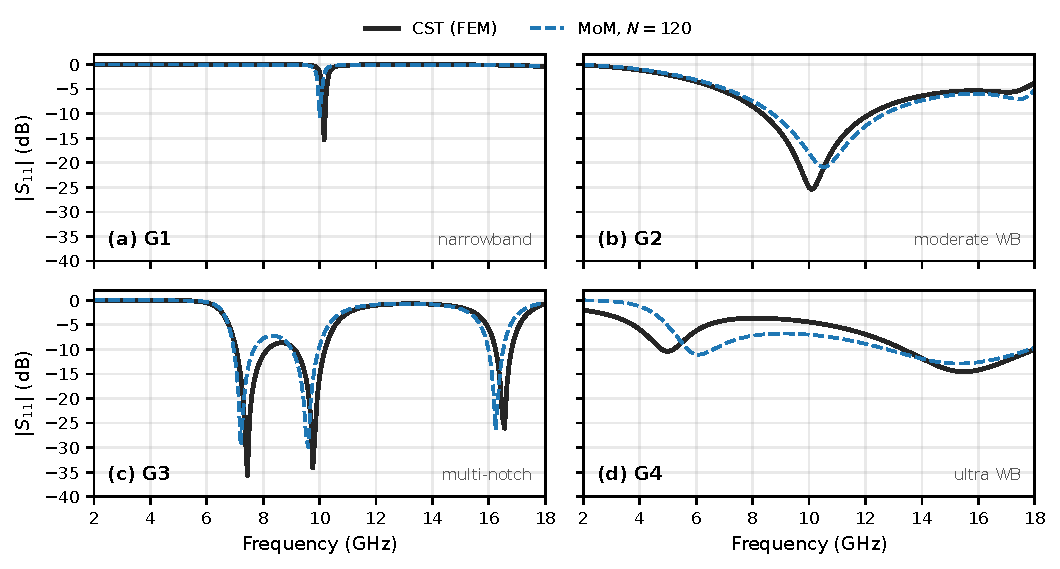
\includegraphics[width=0.95\textwidth]{fig_validation.pdf}
		\caption{Comparison of $|S_{11}|$ (dB) computed by the proposed solver
			($N=120$) and by the commercial FEM solver for (a)~G1, (b)~G2, (c)~G3
			and (d)~G4.}
		\label{fig:validation}
	\end{figure*}
	
	\begin{table}[t]
		\centering
		\caption{Resonant Notches: FEM (CST) vs Proposed Solver ($N=120$)}
		\label{tab:valid}
		\small
		\setlength{\tabcolsep}{3.5pt}
		\begin{tabular*}{\columnwidth}{@{\extracolsep{\fill}}c c c c c c c@{}}
			\hline
			& & \multicolumn{2}{c}{$f_{\mathrm{notch}}$ (GHz)} & & \multicolumn{2}{c}{Depth (dB)}\\
			Geom. & Notch & FEM & MoM & $\Delta f$ (\%) & FEM & MoM\\
			\hline
			G1 & 1 & 10.16 & 10.00 & $-1.57$ & $-15.31$ & $-10.58$\\
			G2 & 1 & 10.08 & 10.56 & $+4.76$ & $-25.41$ & $-20.87$\\
			G3 & 1 & 7.44 & 7.20 & $-3.23$ & $-35.65$ & $-29.46$\\
			G3 & 2 & 9.76 & 9.60 & $-1.64$ & $-34.15$ & $-29.90$\\
			G3 & 3 & 16.56 & 16.24 & $-1.93$ & $-26.06$ & $-26.32$\\
			G4 & 1 & 15.52 & 15.36 & $-1.03$ & $-14.57$ & $-12.90$\\
			\hline
		\end{tabular*}

		\vspace{2pt}
		{\raggedright\footnotesize $\Delta f=(f_{\mathrm{MoM}}-f_{\mathrm{FEM}})/f_{\mathrm{FEM}}$.
			G4 also has a weaker first dip (FEM 4.96~GHz, MoM 6.08~GHz).\par}
	\end{table}
	
	\subsection{GMRES Iterations}
	
	The spectra in Fig.~\ref{fig:validation} and Table~\ref{tab:valid} use
	$N=120$. Fig.~\ref{fig:conv} shows GMRES iterations on G1: they stay in the
	30--80 range off resonance and rise to about 1600 at the notch, so a
	contiguous frequency block that contains the resonance can take much longer
	than a block away from it. Resistive sheets G2 and G4 stay at or below 80
	iterations across the band, so the spike is a copper-notch effect rather than
	a property of every geometry.
	
	\subsection{Performance}
	
	Table~\ref{tab:perf} reports 201-point sweep times
	($N=120$, 2--18~GHz): the HPC A100 is $33\times$--$50\times$ faster than the
	CPU FFT-MoM and $24\times$--$253\times$ faster than CST. Scaled to a
	1000-geometry dataset, the mean sweep times project to about 37~h for CST,
	12~h for the CPU FFT-MoM and 17~min on the A100 (Fig.~\ref{fig:scaling}).
	
	\begin{table}[t]
		\centering
		\caption{Runtime for One 201-Point Sweep ($N=120$, 2--18~GHz)}
		\label{tab:perf}
		\small
		\begin{tabular*}{\columnwidth}{@{\extracolsep{\fill}}lrrrrr@{}}
			\hline
			& & & & \multicolumn{2}{c}{A100 speedup}\\
			& CST (s) & CPU (s) & A100 (s) & vs CPU & vs CST\\
			\hline
			G1 & 182 & 24 & 0.72 & $33\times$ & $253\times$\\
			G2 & 199 & 41 & 1.06 & $39\times$ & $188\times$\\
			G3 & 117 & 44 & 1.07 & $41\times$ & $109\times$\\
			G4 & 29 & 61 & 1.23 & $50\times$ & $24\times$\\
			\hline
		\end{tabular*}

		\vspace{2pt}
		{\raggedright\footnotesize HPC NVIDIA A100. CPU: same FFT-MoM,
			NumPy/SciPy, complex128.\par}
	\end{table}

	\begin{figure}[t]
		\centering
		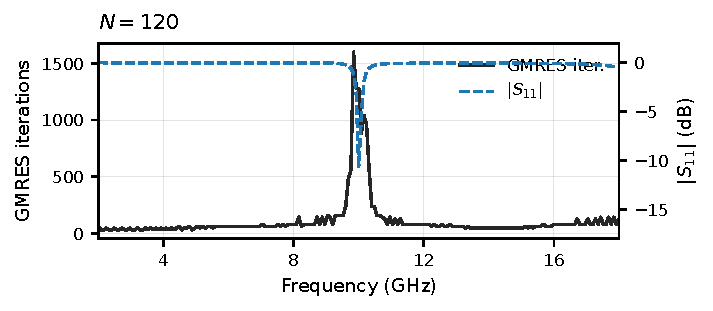
\includegraphics[width=0.92\columnwidth]{fig_conv.pdf}
		\caption{GMRES iteration count across the $N=120$ sweep of G1, with
			$|S_{11}|$ on the right axis.}
		\label{fig:conv}
		\vspace{6pt}
		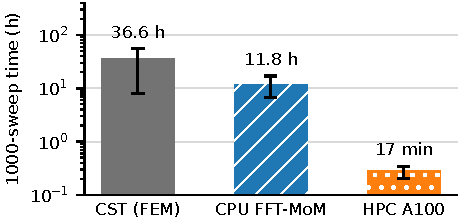
\includegraphics[width=0.78\columnwidth]{fig_scaling.pdf}
		\caption{Projected wall-clock time for 1000 sweeps
			(201 points each, $N=120$, 2--18~GHz), taken as 1000 times the
			measured single-sweep time. Bars show the mean over G1--G4; whiskers
			span the fastest and slowest geometry.}
		\label{fig:scaling}
	\end{figure}

	% Flush every figure and table so the Conclusion starts after them.
	\FloatBarrier
	\raggedbottom
	\section{Conclusion}
	\label{sec:concl}
	
	A spectral-domain MoM solver for metasurface absorbers on grounded substrates
	has been presented. Folding the slab and ground into closed-form TE/TM Floquet
	Green's functions and applying the operator with FFTs avoids a dense impedance
	matrix; GMRES on the GPU reduces a full sweep by up to $50\times$ relative to
	the same algorithm on the CPU. Principal notches agree with commercial FEM to
	within $4.8\%$ in frequency (depths within $6.2$~dB). The residual error has
	not yet been separated by cause; likely contributors are the staircase
	approximation of curved edges, Floquet aliasing, and the zero-thickness
	sheet model. Future work includes oblique incidence, multilayer stacks, and
	training-data generation.
	
	\balance
	\begin{thebibliography}{99}
		
		\bibitem{munk2000}
		B.~A.~Munk, \emph{Frequency Selective Surfaces: Theory and Design}.
		New York, NY, USA: Wiley, 2000.
		
		\bibitem{joy2021}
		V.~Joy, A.~Dileep, P.~V.~Abhilash, R.~U.~Nair, and H.~Singh, ``Metasurfaces
		for stealth applications: A comprehensive review,'' \emph{J. Electron.
			Mater.}, vol.~50, pp.~3129--3148, 2021.
		
		\bibitem{cst}
		Dassault Syst\`emes, \emph{CST Studio Suite}. [Online]. Available:
		https://www.3ds.com
		
		\bibitem{liu2018}
		D.~Liu, Y.~Tan, E.~Khoram, and Z.~Yu, ``Training deep neural networks for the
		inverse design of nanophotonic structures,'' \emph{ACS Photon.}, vol.~5,
		no.~4, pp.~1365--1369, 2018.
		
		\bibitem{ma2018}
		W.~Ma, F.~Cheng, and Y.~Liu, ``Deep-learning-enabled on-demand design of
		chiral metamaterials,'' \emph{ACS Nano}, vol.~12, no.~6, pp.~6326--6334, 2018.
		
		\bibitem{harrington}
		R.~F.~Harrington, \emph{Field Computation by Moment Methods}.
		New York, NY, USA: Macmillan, 1968.
		
		\bibitem{itoh1980}
		T.~Itoh, ``Spectral domain immitance approach for dispersion characteristics
		of generalized printed transmission lines,'' \emph{IEEE Trans. Microw. Theory
			Techn.}, vol.~28, no.~7, pp.~733--736, Jul. 1980.
		
		\bibitem{mittra1988}
		R.~Mittra, C.~H.~Chan, and T.~Cwik, ``Techniques for analyzing frequency
		selective surfaces: A review,'' \emph{Proc. IEEE}, vol.~76, no.~12,
		pp.~1593--1615, Dec. 1988.
		
		\bibitem{cwik1987}
		T.~Cwik and R.~Mittra, ``Scattering from a periodic array of free-standing
		arbitrarily shaped perfectly conducting or resistive patches,'' \emph{IEEE
			Trans. Antennas Propag.}, vol.~35, no.~11, pp.~1226--1234, Nov. 1987.
		
		\bibitem{lezar2010}
		E.~Lezar and D.~B.~Davidson, ``GPU-accelerated method of moments by example:
		Monostatic scattering,'' \emph{IEEE Antennas Propag. Mag.}, vol.~52, no.~6,
		pp.~120--135, Dec. 2010.
		
		\bibitem{glisson1980}
		A.~W.~Glisson and D.~R.~Wilton, ``Simple and efficient numerical methods for
		problems of electromagnetic radiation and scattering from surfaces,''
		\emph{IEEE Trans. Antennas Propag.}, vol.~28, no.~5, pp.~593--603, Sep. 1980.
		
		\bibitem{saad1986}
		Y.~Saad and M.~H.~Schultz, ``GMRES: A generalized minimal residual algorithm
		for solving nonsymmetric linear systems,'' \emph{SIAM J. Sci. Stat. Comput.},
		vol.~7, no.~3, pp.~856--869, 1986.
		
		\bibitem{paszke2019}
		A.~Paszke \emph{et al.}, ``PyTorch: An imperative style, high-performance deep
		learning library,'' in \emph{Adv. Neural Inf. Process. Syst.}, 2019,
		pp.~8024--8035.
		
	\end{thebibliography}
	
\end{document}
